\documentclass[11pt,letterpaper]{article}

\addtolength{\oddsidemargin}{-.875in}
\addtolength{\evensidemargin}{-.875in}
\addtolength{\textwidth}{1.75in}

\addtolength{\topmargin}{-.875in}
\addtolength{\textheight}{1.75in}

\usepackage[utf8]{inputenc}
\usepackage{caption} % for table captions
\usepackage{amsmath} % for multi-line equations and piecewises
\DeclareMathOperator{\sign}{sign}
\usepackage{graphicx}
\usepackage{relsize}
\usepackage{xspace}
\usepackage{verbatim} % for block comments
\usepackage{subcaption} % for subfigures
\usepackage{enumitem} % for a) b) c) lists
\newcommand{\Cyclus}{\textsc{Cyclus}\xspace}%
\newcommand{\Cycamore}{\textsc{Cycamore}\xspace}%
\newcommand{\deploy}{\texttt{d3ploy}\xspace}%
\newcommand{\Deploy}{\texttt{D3ploy}\xspace}%
\usepackage{tabularx}
\usepackage{color}
\usepackage{multirow}
\usepackage{float} 
\usepackage[acronym,toc]{glossaries}
%\include{acros}
\definecolor{bg}{rgb}{0.95,0.95,0.95}
\newcolumntype{b}{X}
\newcolumntype{f}{>{\hsize=.15\hsize}X}
\newcolumntype{s}{>{\hsize=.5\hsize}X}
\newcolumntype{m}{>{\hsize=.75\hsize}X}
\newcolumntype{r}{>{\hsize=1.1\hsize}X}
\usepackage{titling}
\usepackage[hang,flushmargin]{footmisc}
\renewcommand*\footnoterule{}
\usepackage{tikz}

\usetikzlibrary{shapes.geometric,arrows}
\tikzstyle{process} = [rectangle, rounded corners, 
minimum width=1cm, minimum height=1cm,text centered, draw=black, 
fill=blue!30]
\tikzstyle{arrow} = [thick,->,>=stealth]

\graphicspath{}
\title{Nitrogen fertilizers}
%\author{Roberto E. Fairhurst Agosta}

\begin{document}
%	\begin{titlepage}
%		\maketitle
%		\thispagestyle{empty}
%	\end{titlepage}

\section{Different types of fertilizers}
Nitrogen based: anhydrous ammonia, urea, ammonium nitrate, UAN solution, ammonium sulfate.
Phosphorus based: diammonium phosphate, monoammonium phosphate, triple super phosphate, ordinary super phosphate, ammonium polyphosphate.
Potassium based: potassium chloride, potassium sulfate, potassium nitrate \cite{hugh_savoy_fertilizers_2009}.

We will focus on nitrogen fertilizers as they represent a major industry worldwide \cite{guichon_valves_nitrogen_2020} and uses hydrogen in its production process.

\section{Nitrogen Fertilizers}
Nitrogen fertilizers include many types of liquid and solid products, among which the most common are ammonia, ammonium nitrate, and urea \cite{guichon_valves_nitrogen_2020}.

A reaction of nitrogen from the air with hydrogen from natural gas at high pressure and temperature produces ammonia by means of the Haber process (200-300 bars and 450$^{\circ}$C).

For ease of handling, other types of fertilizers are preferable, see Figure \ref{fig:nitrof}.

\begin{figure}[] %use H
	\centering
	\includegraphics[width=\linewidth]{figures/guichon.png}
	\hfill
	\caption{\cite{guichon_valves_nitrogen_2020}.}
	\label{fig:nitrof}
\end{figure}

\section{Haber Process}
Haber invented a large-scale catalytic synthesis process of ammonia by using high pressure and temperature (150-200 atm and 500$^{\circ}$C), and an iron catalyst. Bosch developed suitable high-pressure equipment and production methods for large-scale production of ammonia.
Nowadays, the worldwide production of ammonia exceeds 130 million tonnes \cite{modak_haber_2011}.

The reaction 
\begin{equation}
N_2 + 3 H_2 \leftrightarrow 2 NH_3; \Delta H_{298K}=-45.7kJ/mol
\end{equation}
describes the synthesis of ammonia from nitrogen and hydrogen. The formation of ammonia is an exothermic reaction. Temperature and pressure affect the mole fraction of ammonia produced as shown in Figure \ref{fig:hbpt}.

\begin{figure}[] %use H
	\centering
	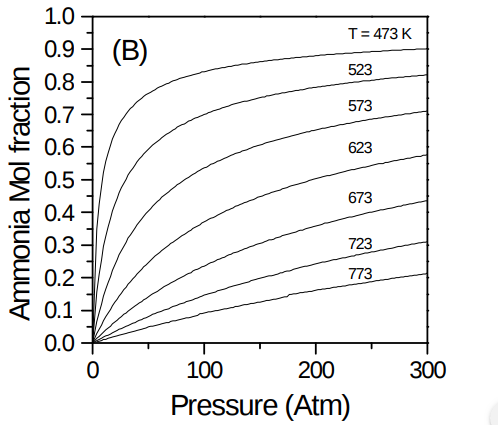
\includegraphics[width=\linewidth]{figures/haberbosch.png}
	\hfill
	\caption{Mole fraction of ammonia at different pressures for fixed values of temperature \cite{modak_haber_2011}.}
	\label{fig:hbpt}
\end{figure}

The reaction does not proceed at ambient temperature because nitrogen requires a lot of energy to dissociate. The presence of the iron catalyst reduces the activation energy reducing the temperature reaction conditions. The process needs high temperatures, ranging from 250 to 400 ${\circ}$C, to dissociate the N$_2$ and H$_2$ \cite{modak_haber_2011}. Figure \ref{fig:hbpt2} displays contours of reaction rate in the phase plane of conversion of reactants and temperature. (Note to my future self: conversion rate is the efficiency of the process, not all the H$_2$ and the N$_2$ react, just a percentage of it.)

\begin{figure}[] %use H
	\centering
	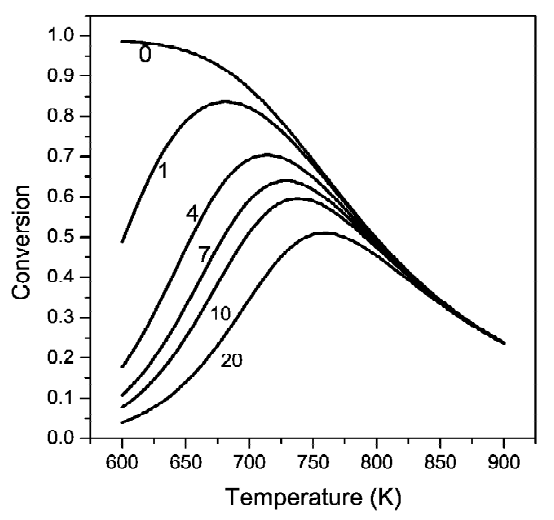
\includegraphics[width=\linewidth]{figures/haberbosch2.png}
	\hfill
	\caption{Contours of constant reaction rate (kg/m$^3$catalyst/hr) \cite{modak_haber_2011}.}
	\label{fig:hbpt2}
\end{figure}



\pagebreak
\bibliographystyle{plain}
\bibliography{bibliography}

\end{document}
